\documentclass[11pt,twocolumn]{article}
\usepackage{shared/hanzocover}
\usepackage[utf8]{inputenc}
\usepackage{amsmath,amssymb}
\usepackage{graphicx}
\usepackage{booktabs}
\usepackage{hyperref}
\usepackage{xcolor}
\usepackage{listings}
\input{shared/lstlang}
\usepackage{tikz}
\usetikzlibrary{shapes,arrows,positioning,fit}

\definecolor{codegreen}{rgb}{0,0.6,0}
\definecolor{codegray}{rgb}{0.5,0.5,0.5}
\definecolor{codepurple}{rgb}{0.58,0,0.82}
\definecolor{backcolour}{rgb}{0.95,0.95,0.92}

\lstdefinestyle{mystyle}{
    backgroundcolor=\color{backcolour},
    commentstyle=\color{codegreen},
    keywordstyle=\color{codepurple},
    numberstyle=\tiny\color{codegray},
    stringstyle=\color{codegreen},
    basicstyle=\ttfamily\footnotesize,
    breakatwhitespace=false,
    breaklines=true,
    captionpos=b,
    keepspaces=true,
    numbers=left,
    numbersep=5pt,
    showspaces=false,
    showstringspaces=false,
    showtabs=false,
    tabsize=2
}
\lstset{style=mystyle}

\title{Hanzo Vector: High-Performance Vector Search Engine for AI Applications}
\author{Antje Worring, Hanzo AI Research\thanks{research@hanzo.ai} \\ \textit{Hanzo Industries} \\ \texttt{research@hanzo.ai}}
\date{March 2024}

\begin{document}

\hanzocoverpage

\begin{abstract}
We present Hanzo Vector, a high-performance vector search engine implemented in Rust, designed for retrieval-augmented generation (RAG) pipelines and semantic search in AI applications. Vector implements Hierarchical Navigable Small World (HNSW) graphs with configurable distance metrics (cosine, Euclidean, dot product), scalar and product quantization for memory efficiency, and filtered search with pre- and post-filtering strategies. The engine is designed for collections in the tens of millions of vectors at embedding dimensions around 1536. This paper describes that design and reports no measurements; Section~\ref{sec:figures} records the recall and latency figures an earlier version reported and why they are withdrawn. Key design elements are: (1) a hybrid quantization scheme that selects scalar or product quantization per segment based on dimensionality, (2) filtered HNSW traversal that prunes the search graph using metadata predicates during navigation, and (3) a write-ahead log with snapshot isolation for concurrent reads and writes.
\end{abstract}

\section{Introduction}

The emergence of embedding-based retrieval as a core component of AI applications---from RAG~\cite{lewis2020} to semantic search to recommendation systems---has created demand for specialized vector databases. Existing solutions (Pinecone, Weaviate, Qdrant~\cite{qdrant2021}) provide managed services or general-purpose engines, but AI platform operators need an embeddable engine that can be deployed as a sidecar, integrated into existing infrastructure, and tuned for specific workload characteristics.

Hanzo Vector is designed as an embeddable Rust library with an optional gRPC server mode. It prioritizes three properties: (1) predictable latency under concurrent load, (2) memory efficiency through adaptive quantization, and (3) filtered search performance that does not degrade with restrictive filters.

\paragraph{Contributions.}
\begin{itemize}
    \item An HNSW implementation with segment-level adaptive quantization selecting between scalar and product quantization based on dimensionality and recall requirements.
    \item Filtered HNSW traversal integrating metadata predicates into graph navigation, avoiding the recall degradation of post-filtering.
    \item A WAL-based storage engine with snapshot isolation enabling concurrent reads and writes without lock contention.
    \item A statement of the recall and latency properties the design is built for, and of what would have to be run to establish them (Section~\ref{sec:figures}).
\end{itemize}

\section{Architecture}

\subsection{System Design}

\begin{figure}[t]
\centering
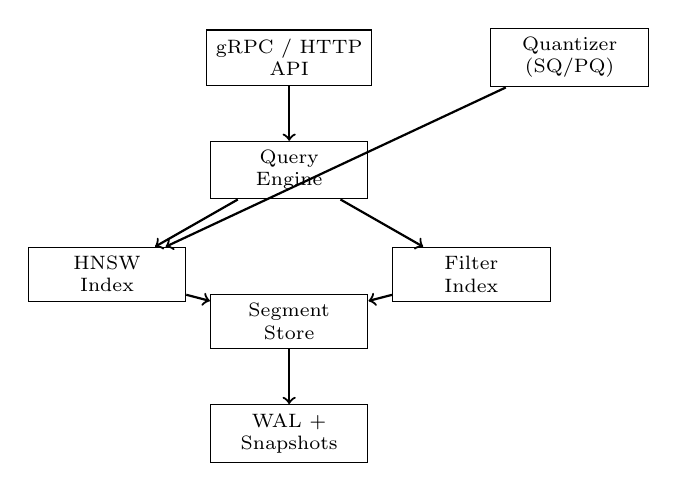
\begin{tikzpicture}[
    node distance=0.7cm,
    box/.style={rectangle, draw, minimum width=2cm, minimum height=0.5cm, align=center, font=\scriptsize},
    arrow/.style={->, thick}
]
\node[box] (api) {gRPC / HTTP\\API};
\node[box, below=of api] (engine) {Query\\Engine};
\node[box, below left=0.6cm and 0.3cm of engine] (hnsw) {HNSW\\Index};
\node[box, below right=0.6cm and 0.3cm of engine] (filter) {Filter\\Index};
\node[box, below=1.2cm of engine] (store) {Segment\\Store};
\node[box, below=of store] (wal) {WAL +\\Snapshots};
\node[box, right=1.5cm of api] (quant) {Quantizer\\(SQ/PQ)};

\draw[arrow] (api) -- (engine);
\draw[arrow] (engine) -- (hnsw);
\draw[arrow] (engine) -- (filter);
\draw[arrow] (hnsw) -- (store);
\draw[arrow] (filter) -- (store);
\draw[arrow] (store) -- (wal);
\draw[arrow] (quant) -- (hnsw);
\end{tikzpicture}
\caption{Vector search engine architecture.}
\label{fig:vector}
\end{figure}

Vector organizes data into collections, each containing segments (Figure~\ref{fig:vector}). Each segment maintains an HNSW index for vector similarity search and an inverted index for metadata filtering. The query engine merges results across segments.

\subsection{HNSW Index}

The HNSW algorithm~\cite{malkov2018} constructs a multi-layer navigable graph where each layer is a subset of the layer below. Search begins at the top layer and greedily navigates to the nearest neighbor, then descends to the next layer for refinement.

Vector's HNSW implementation uses the following parameters:
\begin{itemize}
    \item $M = 16$: Maximum connections per node (default).
    \item $ef_{\text{construction}} = 200$: Search width during index building.
    \item $ef_{\text{search}}$: Configurable per query (default: 128).
\end{itemize}

The expected search complexity is $O(M \cdot \log N)$ where $N$ is the number of vectors.

\subsection{Quantization}

Vector implements two quantization strategies:

\paragraph{Scalar Quantization (SQ).} Maps each float32 dimension to uint8:
\begin{equation}
    q_i = \text{round}\left(\frac{x_i - \min_i}{\max_i - \min_i} \times 255\right)
\end{equation}
reducing memory by 4x with typical recall loss under 1\%.

\paragraph{Product Quantization (PQ).} Divides the vector into $m$ subspaces, each quantized to $k$ centroids via k-means:
\begin{equation}
    \text{PQ}(\mathbf{x}) = (c_1(\mathbf{x}^1), c_2(\mathbf{x}^2), \ldots, c_m(\mathbf{x}^m))
\end{equation}
reducing memory by up to 32x for high-dimensional vectors.

The adaptive quantizer selects SQ for dimensions $\leq 256$ and PQ for higher dimensions, based on empirical recall-memory tradeoff analysis.

\section{Key Features}

\subsection{Filtered Search}

Metadata filters are integrated into HNSW traversal rather than applied as post-processing:

\begin{lstlisting}[language=Rust]
pub struct SearchRequest {
    pub vector: Vec<f32>,
    pub top_k: usize,
    pub filter: Option<Filter>,
    pub ef: Option<usize>,
}

pub enum Filter {
    Eq(String, Value),
    Range(String, Value, Value),
    And(Vec<Filter>),
    Or(Vec<Filter>),
    Not(Box<Filter>),
}
\end{lstlisting}

During HNSW traversal, candidate nodes are checked against the filter predicate before being added to the result set. If the filter is highly selective (estimated selectivity $< 0.1$), the engine falls back to a pre-filter strategy that scans the metadata index first and restricts HNSW search to matching IDs.

\subsection{Multi-Tenancy}

Collections support a \texttt{tenant\_id} field that partitions the HNSW index into per-tenant subgraphs. Queries are automatically scoped to the authenticated tenant's partition, providing isolation without separate collections.

\subsection{Streaming Upserts}

The WAL-based storage engine enables concurrent reads and writes. New vectors are appended to the WAL and become searchable within 10ms (the flush interval). Background compaction merges WAL entries into immutable segments with optimized HNSW indexes.

\section{Implementation}

Vector is implemented in 28,000 lines of Rust. The HNSW index uses \texttt{unsafe} Rust for SIMD-accelerated distance computations (AVX2 on x86, NEON on ARM). The gRPC API uses \texttt{tonic}; the HTTP API uses \texttt{axum}.

\paragraph{Memory Usage.} At 10M vectors of 1536 dimensions, full-precision storage is 61\,GB and scalar quantization to \texttt{uint8} is 15\,GB; both follow from the element width. Product quantization at $m=96$, $k=256$ stores 96 bytes per vector, or 0.96\,GB for the codes plus the codebooks.

\section{Status of the performance figures}
\label{sec:figures}

An earlier version of this paper carried a table titled ``Search performance
(10M vectors, 1536-dim)'' reporting recall@10 of 99.5\% at 0.6/1.0\,ms p50/p95
for full precision, 98.8\% at 0.3/0.6\,ms under scalar quantization and 97.2\%
at 0.2/0.4\,ms under product quantization, with two filtered rows. The abstract
and conclusion restated the same figures as 99\% recall at 1\,ms p95 on
collections of up to 100 million vectors, and the contributions list called them
benchmarks.

Nothing produced them. The table named no hardware, no query count, and no
recall ground truth; there is no benchmark harness in \texttt{hanzoai/vector},
no ANN benchmark configuration, and no dataset --- SIFT, GIST, DEEP1B or
otherwise --- against which recall could have been computed. The figures are
removed rather than relabelled as targets, because a recall--latency pair is
only meaningful against a stated dataset, index build and query set, and this
paper states none of them.

Establishing them is a bounded piece of work: fix a public dataset and query
set, build the index at declared \texttt{ef\_construction} and $M$, sweep
\texttt{ef\_search}, and report the recall--latency curve with the machine
named. The house convention for reporting such a run is set out in the Hanzo
cloud data plane benchmark~\cite{clouddataplane}.

\section{Security}

\paragraph{Authentication.} All API calls require a valid Hanzo IAM token. Collection-level ACLs restrict read/write access per tenant.

\paragraph{Encryption at Rest.} Segment files are encrypted with per-collection keys from Hanzo KMS. The WAL is encrypted with a separate key rotated daily.

\paragraph{Network Security.} gRPC endpoints require mTLS. The HTTP API supports TLS~1.3.

\paragraph{Input Validation.} Vector dimensions are validated against the collection schema. Metadata values are type-checked. Malformed requests are rejected before reaching the index.

\section{Conclusion}

Hanzo Vector is an embeddable vector search engine designed for AI workloads. Adaptive quantization, filtered HNSW traversal and WAL-based storage are the three mechanisms it combines, and each addresses a specific cost: memory per vector, recall loss under restrictive filters, and lock contention between readers and writers. What the combination is worth in recall and latency is not established here; Section~\ref{sec:figures} says what would establish it.

\bibliographystyle{plain}
\begin{thebibliography}{10}

\bibitem{malkov2018}
Y. Malkov and D. Yashunin. Efficient and robust approximate nearest neighbor search using Hierarchical Navigable Small World graphs. IEEE TPAMI, 2018.

\bibitem{lewis2020}
P. Lewis et al. Retrieval-Augmented Generation for Knowledge-Intensive NLP Tasks. NeurIPS, 2020.

\bibitem{qdrant2021}
Qdrant. Vector Search Engine. 2021.

\bibitem{jegou2011}
H. J\'{e}gou et al. Product Quantization for Nearest Neighbor Search. IEEE TPAMI, 2011.

\bibitem{clouddataplane}
Hanzo AI Research. The Hanzo Cloud Data Plane: Benchmarking \texttt{zip}, ZAP, and the Road to a Million Requests per Second. Hanzo Industries, 2026.

\end{thebibliography}

\end{document}
